\documentclass[aspectratio=169, table]{beamer}
\usepackage[utf8]{inputenc}
\usepackage{xcolor}

\usepackage{multicol}
\usepackage{booktabs}
\usepackage{arydshln}
\usepackage[abs]{overpic}
\usepackage{tikz}
\usetikzlibrary{fadings}
%\usepackage{enumitem}
%\usepackage[table]{xcolor} 

\usepackage{empheq}

\definecolor{redp}{rgb}{0.78, 0.03, 0.08}
\definecolor{greenp}{rgb}{0.0, 0.51, 0.5}
\definecolor{yellowp}{rgb}{0.59, 0.44, 0.09}
\definecolor{greencol}{rgb}{0.0,0.4,0.0}
\definecolor{fcolor}{rgb}{0.8, 0.4, 0.0}
\definecolor{bluep}{rgb}{205,219,194}

\newcommand{\enb}[1]{\textcolor{poliblue1}{\textbf{#1}}}
\newcommand{\eno}[1]{\textcolor{orangep}{\textbf{#1}}}
\definecolor{softblue}{cmyk}{.2, .1, .1, .2}
\newcommand{\soft}[1]{\textcolor{softblue}{#1}}

\title{Optimistic Policy Optimization via Multiple Importance Sampling}
\date[AAA]{\vspace{0.2cm} \\ \small{ 11th June 2019 \\ Thirty-sixth International Conference on Machine Learning, Long Beach, CA, {USA}}}
\author[M. Papini]{\textbf{Matteo Papini} \quad Alberto Maria Metelli\\
						\small{Lorenzo Lupo \quad Marcello Restelli}}

\usetheme{polimithx}
\usetikzlibrary{calc}

\usepackage[customcolors,shade]{hf-tikz}

%%%%%%%%%%%%%%%%%%%%%%%%%% BIBLIOGRAPHY
\usepackage{natbib}
\bibliographystyle{apalike}
% make bibliography entries smaller
\renewcommand\bibfont{\scriptsize}
% If you have more than one page of references, you want to tell beamer
% to put the continuation section label from the second slide onwards
\setbeamertemplate{frametitle continuation}[from second]

%CUSTOM COMMANDS

\usepackage[many]{tcolorbox}
\usetikzlibrary{decorations.pathreplacing}
\usetikzlibrary{arrows,shapes}
\usetikzlibrary{positioning}

\usepackage{mymacros}

\begin{document}

\setbeamertemplate{caption}{\raggedright\insertcaption\par}

\begin{frame}[noframenumbering]
\titlepage
\end{frame}

\begin{frame}
\frametitle{Policy Optimization} 
\begin{columns}
\begin{column}{.65\textwidth}
\begin{overlayarea}{\textwidth}{\textheight}
\begin{itemize}
	\setlength{\itemsep}{20pt}
	\item \enb{Parameter space} $\Theta \subseteq \Reals^d$
	\item<2-> A parametric \enb{policy} for each $\vtheta\in\Theta$
	\item<3-> Each inducing a distribution $p_{\vtheta}$ over \enb{trajectories}
	\item<4-> A \enb{return} $R(\tau)$ for every trajectory $\tau$
	\item<5-> {\enb{Goal:} $\max\limits_{\vtheta\in\Theta} J(\vtheta) = \Exp_{\tau\sim p_{\vtheta}}\left[R(\tau)\right]$}
	\item<6-> Iterative optimization (\eg gradient ascent)
\end{itemize}
\end{overlayarea}
\end{column}
\begin{column}{.35\textwidth}
\begin{overlayarea}{\textwidth}{\textheight}
	\only{
	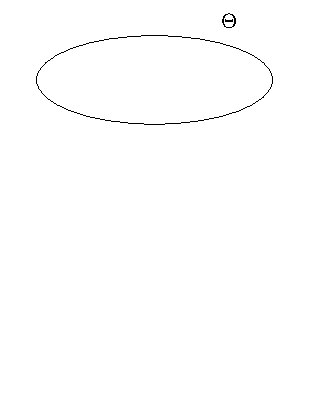
\includegraphics[]{animation/spaces1.pdf}}<1>
	\only{
	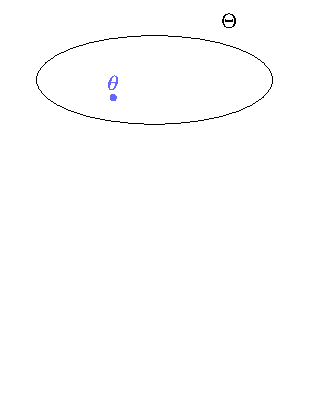
\includegraphics[]{animation/spaces2.pdf}}<2>
	\only{
	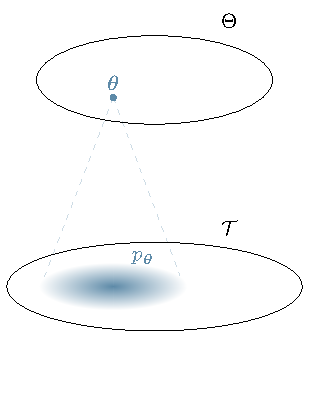
\includegraphics[]{animation/spaces3.pdf}}<3>
	\only{
	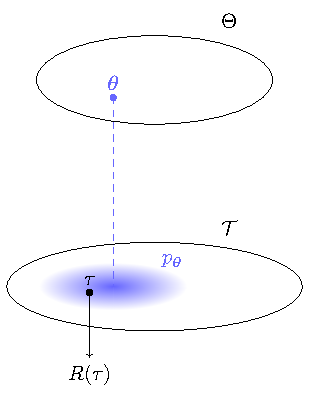
\includegraphics[]{animation/spaces4.pdf}}<4>
	\only{
	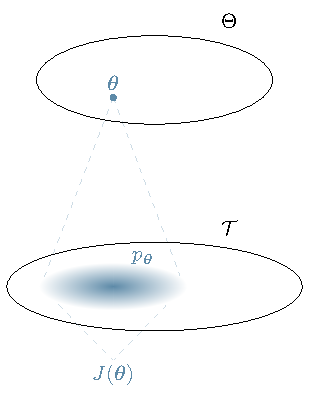
\includegraphics[]{animation/spaces5.pdf}}<5>
	\only{
	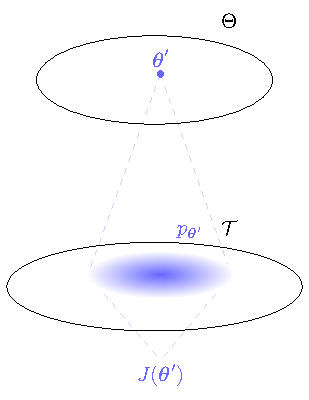
\includegraphics[]{animation/spaces13.pdf}}<6->
\end{overlayarea}
\end{column}
\end{columns}
\end{frame}

\begin{frame} 
\frametitle{Exploration in Policy Optimization}
\begin{overlayarea}{\textwidth}{.75\textheight}
\begin{itemize}
	\setlength{\itemsep}{20pt}
	\item<1-4> \eno{Continuous} decision process $\implies$ difficult\vfill
	\item<2-4> Policy gradient methods tend to be \eno{greedy}~(\eg TRPO~\citep{schulman2015trust}, PGPE~\citep{sehnke2008policy})\vfill
	\item<3-4> Mainly \eno{undirected} (\eg entropy bonus~\citep{haarnoja2018soft})\vfill
	\item<4> \eno{Lack of theoretical guarantees}\vfill
\end{itemize}
\end{overlayarea}
\begin{overlayarea}{\textwidth}{.25\textheight}
\centering
\vspace{-40pt}
\only<5>
{\Large \enb{If only this were a Multi-Armed Bandit...}}
\only<6->
{\Large \enb{If only this were a} \eno{Correlated} \enb{Multi-Armed Bandit...}}
\end{overlayarea}
\end{frame}

\begin{frame} 
\frametitle{Policy Optimization as a Correlated MAB } 
\begin{columns}
\begin{column}{.65\textwidth}
\begin{overlayarea}{\textwidth}{.75\textheight}
\begin{itemize}
	\setlength{\itemsep}{20pt}
	\item<1-> \enb{Arms:} parameters $\vtheta$\vfill
	\item<2-> \enb{Payoff:} expected return $J(\vtheta)$\vfill
	\item<3-> \eno{Continuous MAB}~\citep{kleinberg2013bandits}\only<1>{: we \emph{need} structure}\vfill
	\item<4-> {\enb{Arm correlation}~\citep{pandey2007multi} through trajectory distributions}\vfill
	\item<5-> \enb{Importance Sampling (IS)}
\end{itemize}
\end{overlayarea}
\end{column}
\begin{column}{.65\textwidth}
\begin{overlayarea}{\textwidth}{\textheight}
\only<1>{
	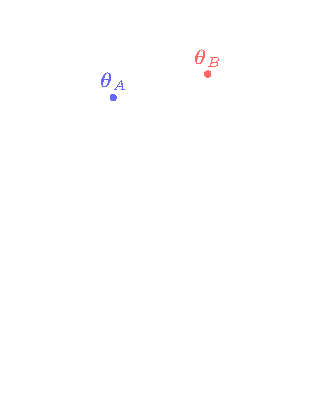
\includegraphics[]{animation/spaces10.pdf}
}
\only<2>{
	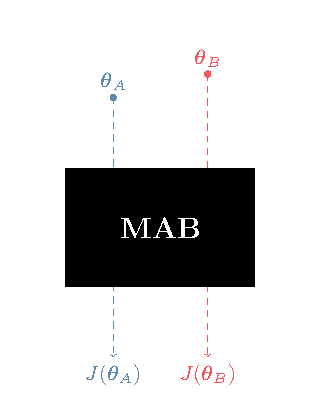
\includegraphics[]{animation/spaces11.pdf}
}
\only<3>{
	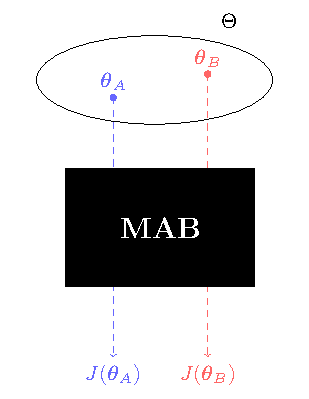
\includegraphics[]{animation/spaces6.pdf}
}
\only<4>{
	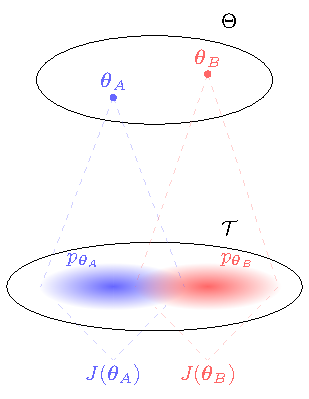
\includegraphics[]{animation/spaces7.pdf}
}
\only<5>{
	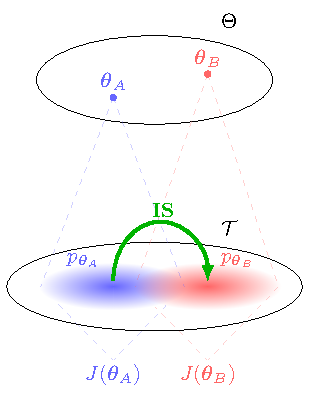
\includegraphics[]{animation/spaces12.pdf}
}
\end{overlayarea}
\end{column}
\end{columns}
\end{frame}

\begin{frame} 
\frametitle{OPTIMIST} 
\begin{overlayarea}{\textwidth}{.5\textheight}
\begin{itemize}
	\setlength{\itemsep}{20pt}
	\item A \enb{UCB-like} index~\citep{lai1985asymptotically}:
	\begin{align*}
	\large
		B_t(\vtheta) \quad =
		\underbrace{\wc{J}_t(\vtheta)}_{\substack{\textbf{ESTIMATE}\\\\\text{a \eno{truncated} \enb{multiple}}\\ \text{ importance sampling estimator~\cite{veach_optimally_1995,bubeck2013bandits}}}}
		\only<1>{\phantom{
			+\qquad
			\underbrace{C\,
				\sqrt{\frac{d_{2}(p_{\vtheta}\|\Phi_{t})\log\frac{1}{\delta_t}}{t}}}_{\substack{\textbf{EXPLORATION BONUS}\\\\\text{\enb{distributional} distance} \\ \text{from previous arms}}}}}
		\only<2->{
		+\qquad
		\underbrace{C\,
		\sqrt{\frac{{\color{orange!80!black}d_{2}(p_{\vtheta}\|\Phi_{t})}\log\frac{1}{\delta_t}}{t}}}_{\substack{\textbf{EXPLORATION BONUS:}\\\\\text{\enb{distributional} distance} \\ \text{from previous solutions}}}}
	\end{align*}
\end{itemize}
%\only<1-2>{
%	\begin{align*}
%		&\wc{\mu}_t(\vtheta) = \sum_{k=0}^{t-1}
%		\min\left\{M_{t}, \frac{p_{\vtheta}(\tau_k)}
%		{\sum_{j=0}^{t-1}p_{\vtheta_j}(\tau_k)}\right\}R(\tau_k)
%		\only<2>{
%		&\Phi_t = \frac{1}{t}\sum_{k=0}^{t-1}p_{\vtheta_k}
%	}
%	\end{align*}
%}
\end{overlayarea}
\begin{overlayarea}{\textwidth}{.25\textheight}
\only<1>{
	\hspace{.3\textwidth}
	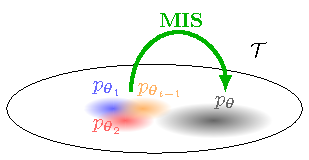
\includegraphics[]{animation/spaces8.pdf}
}
\only<2>{
	\hspace{.3\textwidth}
	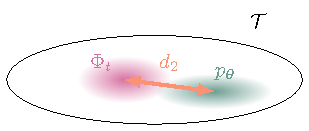
\includegraphics[]{animation/spaces9.pdf}
}
\only<3->{
\vspace{20pt}
\begin{itemize}
	\setlength{\itemsep}{20pt}
	\item Select $\vtheta_t = \arg\max\limits_{\vtheta\in\Theta} B_t(\vtheta)$
\end{itemize}
}
\end{overlayarea}
\end{frame}

\begin{frame} 
\frametitle{Sublinear Regret}
\begin{overlayarea}{\textwidth}{.4\textheight}
\begin{itemize}
	\setlength{\itemsep}{20pt}
	\item<1-> $\mathop{Regret}(T) = \sum_{t=0}^T J(\vtheta^*) - J(\vtheta_t)$
	\vfill
	\item<2-> \enb{Compact}, $d$-dimensional parameter space $\Theta$
	\vfill
	\item<3-> Under \enb{mild assumptions} on the policy class, with high probability:
\end{itemize}
\end{overlayarea}
\LARGE
\begin{align*}
\mathop{Regret}(T) = \wt{\mathcal{O}}\left(\sqrt{dT}\right)
\end{align*}
\end{frame}

\begin{frame}
\frametitle{Empirical Results} 
\begin{columns}
	\begin{column}{.5\textwidth}
		\centering
		{\bf River Swim}
		\begin{figure}
			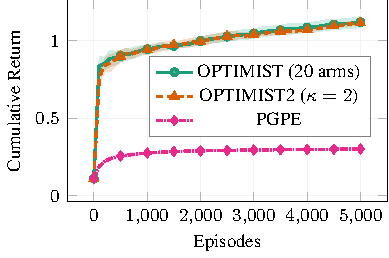
\includegraphics[]{river.pdf}
		\end{figure}
	\end{column}
\hfill
	\begin{column}{.45\textwidth}
		\begin{overlayarea}{\textwidth}{.61\textheight}
		\only<2->{
		\eno{Caveats}
		\begin{itemize}
			\setlength{\itemsep}{10pt}
			\item Easy implementation only for parameter-based exploration~\cite{sehnke2008policy}
			\item Difficult optimization \\$\implies$ discretization
			\item ...
		\end{itemize}}
	\end{overlayarea}
	\end{column}
\end{columns}
\end{frame}

\begin{frame}[plain]
%\frametitle{Thanks} 
\begin{center}
	\huge{\enb{Thank You for Your Attention!}}
\end{center}

\begin{minipage}[]{.5\paperwidth}
	\begin{itemize}
		\item[] Poster \textbf{\#103}
		\item[] Code: \url{github.com/WolfLo/optimist}
		\item[] Contact: matteo.papini@polimi.it
		\item[] Web page: \url{t3p.github.io/icml19} 
	\end{itemize}
\end{minipage}
\hspace{2cm}%
\begin{minipage}[]{.2\paperwidth}
	
\includegraphics[width=\textwidth]{qr.png}
\end{minipage}
\end{frame}


%%%%%%%%%%%%%%%%%%%%%%%%%%%%%%%%%%%%%%%%%%%%%%%%%%%%%%%%%%%%%%%%%%%%%%%%%%%%%%%%%%%%%%%%%
\begin{frame}[allowframebreaks,fragile]
\frametitle{References}
\bibliographystyle{abbrv}
\bibliography{../biblio.bib}
\end{frame}
%%%%%%%%%%%%%%%%%%%%%%%%%%%%%%%%%%%%%%%%%%%%%%%%%%%%%%%%%%%%%%%%%%%%%%%%%%%%%%%%%%%%%%%%%

%%Backup Slides


\end{document}
